\documentclass[a4paper]{article}
\title{Assignment 2}
\author{Student: Harkeerat Singh Sawhney; Student's email: sawhnh@usi.ch}

%%%%%%%%%%%%%%%%%%%
% Packages
%%%%%%%%%%%%%%%%%%
\usepackage{palatino}
\usepackage{amsmath}
\usepackage{bm}
\usepackage{hyperref}
\usepackage{xcolor}
\usepackage{verbatim}
\usepackage{enumerate}
\usepackage{amsmath}
\usepackage{bm}
\usepackage{hyperref}
\usepackage{verbatim}
\usepackage{graphicx}
\usepackage{enumerate}
\usepackage{xcolor}
\usepackage{listings}
\usepackage{listings}
\usepackage{xcolor}
\usepackage{float}
\usepackage{amsmath}
\usepackage{amsmath, amssymb} % for math symbols and fonts
\usepackage{hyperref} % for hyperlinks
\usepackage{listings}
\usepackage{xcolor}
\usepackage{subcaption}

%%%%%%%%%%%%%%%%%%%
% Commands
%%%%%%%%%%%%%%%%%%
\newcommand{\erre}{\mathbf{R}}
\newcommand{\todo}[1]{\textcolor{red}{TODO: #1}}
\newcommand{\link}[2]{\href{#1}{\textcolor{blue}{#2}}}
\definecolor{code}{HTML}{00A99D}
\newcommand{\codeword}[1]{\texttt{\textcolor{code}{#1}}}

\begin{document}
\maketitle

\section{Image classification using CNNs [90/100]}
\subsection{Data (20 pts)}
\begin{enumerate}
	% Load
	\item In this question we were asked to load the dataset through PyTorch and were asked to take some to inspect the data. The dataset was loaded using the \codeword{torchvision.datasets.CIFAR10} function. From the dataset we were able to understand that there were 10 different classes in the dataset. The classes consist of animals and different vehicles. We were able to get 2 different datasets, which is a Train dataset and Test dataset.

	      From the Histogram we were able to observe that in Train Dataset each class has 5000 images whereas in the Test Dataset there is 1000 images per class. The size of each image is 32x32x3. The 3 represents the RGB channels. The Histogram is shown in Figure \ref{fig:question1.1}.

	      \begin{figure}[H]
		      \centering
		      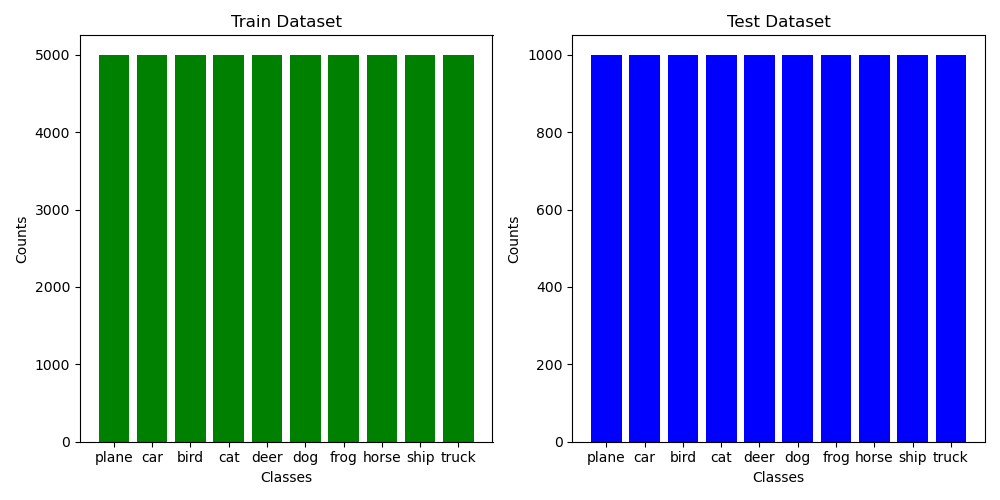
\includegraphics[width=0.8\textwidth]{"../figures/1.1/histogram.png"}
		      \caption{Histogram of the CIFAR10 Dataset(Train and Test)}
		      \label{fig:question1.1}
	      \end{figure}
	\item The Dataset which has been downloaded is not in the correct format which can be used to train a model on.
	      \begin{enumerate}
		      \item Each element in the Dataset is the type of PIL Image for the images while for the labels it is integers.
		      \item In order to convert the dataset to a suitable data type on which we can train a model, we can use \codeword{torchvision.transforms.ToTensor()} function. This function converts the PIL Image to a Tensor. The range of the values in the Tensor is from 0 to 1. The labels are already in the correct format. We are also applying additional normalization to it as well.
		      \item The image itself is supposed to have 3 different dimensions to, in which each dimension defines a characteristic of the image. The image has a dimension of (3,32,32). The first dimension represents the RGB channels, the second dimension represents the height of the image and the third dimension represents the width of the image. However when they are converted to a tensor the dimensions are changed to (4, 3, 32, 32). The additional first dimension is the batch size, which in our case we have kept it to 32.
		      \item The first dimension is the batch size of the images. What it means by batch size of images is that we are going to train the model on 4 images at a time. The main reason for this is that it is computationally more expensive to train the model on 1 image at a time. The second dimension as mentioned before is the RGB channels. The third and fourth dimension are the height and width of the image respectively.
	      \end{enumerate}
	      % Normalization
	\item As the question asked us to convert the dataset to tensor shape of (3, 32, 32) and to have the Standard Deviation of 1 and Mean of 0. In order to do this we first calculate the mean and standard deviation. We do this separately for each chanel (Red, Green, Blue). We then use these values to define normalization through \codeword{transforms.Compose}. We then apply this normalization to the training and testing dataset and calculate the mean and std again to confirm if the normalization has been applied or not.

	      \begin{table}[H]
		      \centering
		      \begin{tabular}{|l|l|l|}
			      \hline
			      \textbf{Channel} & \textbf{Mean} & \textbf{Std Deviation} \\
			      \hline
			      Red              & 0.4914        & 0.2470                 \\
			      Green            & 0.4822        & 0.2435                 \\
			      Blue             & 0.4465        & 0.2616                 \\

			      \hline
		      \end{tabular}
		      \caption{Mean and Standard Deviation of the CIFAR10 Dataset before Normalization}
		      \label{tab:question1.4}
	      \end{table}

	      In Table \ref{tab:question1.4} we can see that the mean and standard deviation of the dataset before normalization while in Table \ref{tab:question1.1.1.4} we can see that the mean and standard deviation of the dataset after normalization. We can see that the mean is 0 and the standard deviation is 1.

	      \begin{table}[H]
		      \centering
		      \begin{tabular}{|l|l|l|}
			      \hline
			      \textbf{Channel} & \textbf{Mean} & \textbf{Std Deviation} \\
			      \hline
			      Red              & 0.0           & 1.0                    \\
			      Green            & 0.0           & 1.0                    \\
			      Blue             & 0.0           & 1.0                    \\

			      \hline
		      \end{tabular}
		      \caption{Mean and Standard Deviation of the CIFAR10 Dataset after Normalization}
		      \label{tab:question1.1.4}
	      \end{table}



	\item In this question we were asked to create a Validation Dataset which would be used for hyperparameter tuning. The ratio is supposed to be of 80:20. I used function trainTestSplit() to get the indicies, which I later used with the subset to create new train set and a valuation set. I then loaded them useing DataLoader which let me later use it during the training of the model.


\end{enumerate}

\subsection{Model (10 pts)}
We were asked to design a Convolutional Neural Network (CNN) architecture implemented in PyTorch. The architecture consists of 3 Convolutional layers, 1 max Pooling Layer, Three fully connected layers, an Activation Function and lastly a Flattening Operation.

The first Convolutional layer took as an input 3 channels and applied 32 filters of the size of 5x5 with a stride of 1 and padding of 2. Then in the second layer it took the 32-chanel output from the first layer and applied 64 filters to it with the same size, stride and padding. Lastly the third layer took 64-channel output from the second layer. and applied 128 filters to it. Again for the last layer it had same size, stride and padding.

A pooling layer is a layer which is used to reduce the spatial size of the input. It applied a 2x2 max pooling operation with a stride of 2.

The activation function which was used is a RelU activation function. The reason for using this activation function is that it is computationally less expensive than other activation functions.

The forward method defined the forward pass of the input through the architecture. The input is passed through the convolutional layers, pooling layer, activation function and then the fully connected layers. The output of the last fully connected layer is then returned.

\subsection{Training (60 pts)}
\begin{enumerate}
	\item The training loop is a standard loop which is very similar to the previouse project. First the model is trained for a specific epoch (in this case 15) and it uses Stochastic Gradient Descent as the optimizer and Cross Entropy Loss as the loss function. For each epoch the model is set to the training mode while running loss and accuracy is calculated over the training data. For each batch of the data of the training set forward pass is performed from the CNN class just defined. The loss is calculated and the gradient is then backpropagated. Finaly the optimzer updates the model parameters. The model is then set to evaluation mode and the validation accuracy is calculated in the same way except the backpropagattion and the optimizer update is not performed. The training and validation accuracy is then printed in the terminal.
	\item After running the training loop for 15 epoch I was able to get the following results:
	      \begin{table}[H]
		      \centering
		      \begin{tabular}{|l|l|l|}
			      \hline
			      \textbf{Training Accuracy} & \textbf{Valuation Accuracy} & \textbf{Test Accuracy} \\
			      \hline
			      87.641                     & 73.590                      & 73.220                 \\

			      \hline
		      \end{tabular}
		      \caption{Accuracy of the Original Model}
		      \label{tab:question1.3.1}
	      \end{table}

	      As it can be see from the Table \ref{tab:question1.3.1} that the model had the Test Accuracy of 73\%. Every Epoch the Training Accuracy and Valuation Accuracy is printed in the terminal as it was asked.
	\item The parameters of the trained module are saved as a \codeword{harkeerat\_sawhney\_1.pth} file.
	\item  We were asked to plot the evolution of the train and validation loss.

	      \begin{figure}[H]
		      \centering
		      \includegraphics[width=0.8\textwidth]{"../figures/1.3/loss_accuracy.png"}
		      \caption{Left: Loss, Right: Accuracy (Original CNN)}
		      \label{fig:question1.3.1}
	      \end{figure}

	      In Figure \ref{fig:question1.3.1} we can see that both train loss valuation loss is decreasing. However while Train loss is decreasing much more consistent manner, the Valuation Loss fluctuates and decreases in an inconsistent manner. One of the reasons for this can be is that the model is overfitting on the training data. This is why the performance on the valuation set is not as good as the training set. This can be seen by looking at the accuracy as well. The accuracy of the training set is much higher than the accuracy of the valuation set. This is a clear indication that the model is overfitting on the training data. The simplicity of the model makes it perform not as well in other cases, and this is why on the Test Set it is 73\% accurate.

	\item  We are asked to now change the architecture and to increase the accuracy as much as we can. The first big change was to create a new CNN Architecture. The are many changes to this, aiming to address the weakness of the previous architecture.

	      The first difference is the number of convolutional layer. I have added 2 more layer, making it 5, to which the purpose was for it learn more complex features. This also includes 2 Dropout Layers, which the main aim was to avoid overfitting. With this it randomly sets a fraction of the input to 0 after each training time. This new architecture also uses GELU (GAussian Error Linear Unit) as the activation function as I read that it is better for such classification tasks. I did try to use different optimizers, however I did not receive any better results anywhere.

	      Another big difference is that the epoch is set to 20. The main reason for this is to see if the model can learn more complex features from the data.

		  \begin{figure}[H]
			\centering
			\includegraphics[width=0.8\textwidth]{"../figures/1.4/loss_accuracy.png"}
			\caption{Left: Loss, Right: Accuracy (New CNN)}
			\label{fig:question1.4.1}
		\end{figure}

		In Figure \ref{fig:question1.4.1} we can see that both train loss valuation loss is decreasing. As compare to the previous architecture the training loss and valuation loss is decreasing in the same constant manner. This means that the new architectue has shown improvement in terms of avoiding overfitting.


		\begin{table}[H]
			\centering
			\begin{tabular}{|l|l|l|}
				\hline
				\textbf{Training Accuracy} & \textbf{Valuation Accuracy} & \textbf{Test Accuracy} \\
				\hline
				94.875                     & 96.020                      & 75.460                 \\

				\hline
			\end{tabular}
			\caption{Accuracy of the New Model}
			\label{tab:question1.5.1}
		\end{table}

		However if we look at the Table \ref{tab:question1.5.1} we can see that the Test Accuracy has not improved significantly. This means that they are still many things which could have been done to improve the model as a whole. 

	\item The parameters of the trained module are saved as a \codeword{harkeerat\_sawhney\_2.pth} file.
\end{enumerate}



% Bonus
\subsection{Bonus question* (5 pts)}
Due to Technical Difficulties I was not able to complete this question.

\section*{Questions [5 points]}
The main idea in this chapter is that to ensure that adding layers to a neural network not only increases its complexity but also enhances its expressiveness. Through the concept of function classes and the use of nested functions classes we can guarantee a increase in expressive power. ResNet is such example which addresses this by introduction residual blocks, where each layer should easily contain the identity function as one of is elements. 

Residual blocks in ResNet consists of shortcut connections that allows the input the bypass some layers which makes it easier for the train-deep networks. ResNetXT is an extnesion of ResNet. There are also trade-off between nonlinearlity and dimensionality withing a block. Increasing Nonlineraity increases the expressive power of the block, however it also increases the dimensionality of the block. This is why ResNetXT uses a bottleneck design which reduces the dimensionality of the block. This is done by using 1x1 convolutions. This allows the network to have more layers while keeping the computational cost low.

\section*{Creating a New Conda Environment with Libraries}

To create a new Conda environment and install libraries from a text file, follow these steps:

\begin{enumerate}
    \item Open your terminal or command prompt.
    
    \item Create a new Conda environment using the following command:
    
    \begin{verbatim}
    conda create --name new_environment_name
    \end{verbatim}
    
    Replace \texttt{new\_environment\_name} with the desired name for your new environment.
    
    \item Activate the new environment:
    
    \begin{verbatim}
    conda activate new_environment_name
    \end{verbatim}
    
    \item Install libraries from the text file using the following command:
    
    \begin{verbatim}
    conda install --file environment.txt
    \end{verbatim}
    
    
\end{enumerate}

Now, your new Conda environment should be set up with the specified libraries

\end{document}